\documentclass[tikz, convert={outfile=\jobname.png}]{standalone}
\usepackage[utf8]{inputenc}
\usetikzlibrary{calc,shapes.multipart,chains,scopes,arrows}

\newcommand{\connectlist}[2]{%
  \draw[*->] let \p1 = (#1.two), \p2 = (#1.center) in (\x1, \y2) -- (#2)}

\newcommand{\oldconnectlist}[2]{%
  \draw[dashed, *->, color=gray] let \p1 = (#1.two), \p2 = (#1.center) in (\x1, \y2) -- (#2)}

\newcommand{\newconnectlist}[2]{%
  \draw[*->, color=red] let \p1 = (#1.two), \p2 = (#1.center) in (\x1, \y2) -- (#2)}

\newcommand{\connectpointer}[2]{%
  \draw[->] (#1) -- (#2)}

\newcommand{\oldconnectpointer}[2]{%
  \draw[dashed, ->, color=gray] (#1) -- (#2)}

\newcommand{\newconnectpointer}[2]{%
  \draw[->, color=red] (#1) -- (#2)}

\begin{document}
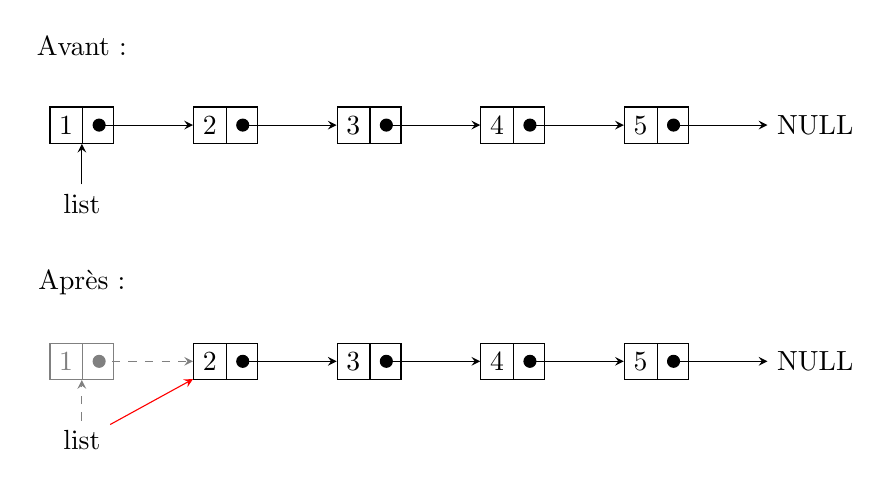
\begin{tikzpicture}[
    list/.style={rectangle split, rectangle split parts=2, draw,
    rectangle split horizontal}, >=stealth]
  \node (before) {Avant~:};
  {[start chain]
    \node[list, on chain, below of=before] (n1) {1};
    \node[list, on chain] (n2) {2};
    \node[list, on chain] (n3) {3};
    \node[list, on chain] (n4) {4};
    \node[list, on chain] (n5) {5};
    \node[on chain] (nil) {NULL};
    \node[below of=n1] (list) {list};

    \connectpointer{list}{n1};
    \connectlist{n1}{n2};
    \connectlist{n2}{n3};
    \connectlist{n3}{n4};
    \connectlist{n4}{n5};
    \connectlist{n5}{nil};}

  \node[below of=list] (after) {Après~:};
  {[start chain]
    \node[list, on chain, below of=after, color=gray] (n1) {1};
    \node[list, on chain] (n2) {2};
    \node[list, on chain] (n3) {3};
    \node[list, on chain] (n4) {4};
    \node[list, on chain] (n5) {5};
    \node[on chain] (nil) {NULL};
    \node[below of=n1] (list) {list};

    \oldconnectpointer{list}{n1};
    \newconnectpointer{list}{n2};
    \oldconnectlist{n1}{n2};
    \connectlist{n2}{n3};
    \connectlist{n3}{n4};
    \connectlist{n4}{n5};
    \connectlist{n5}{nil};}
\end{tikzpicture}

\end{document}
